%!TEX root = 0_architecture_rapport.tex

% subsection title
\section*{Interpretation. There are many other factors which contribute to a players’ salary besides performance. How does this affect your player’s salaries prediction above?}
\addcontentsline{toc}{section}{Interpretation. There are many other factors which contribute to a players’ salary besides performance. How does this affect your player’s salaries prediction above?}
\label{subsec:3Q4}

\paragraph{Upper-bound or lower-bound coefficients}We use the best model we have, i.e. the model with the points, rebounds and assists. 
We first plot the standard error between the estimate salary and the real salary, with the real salary on the x axis. We can see that our prediction is not very good for low salaries but rather good for high salaries (even if it is normal that the standard error diminishes when the salary increases).
\begin{figure}[h!]
\centering
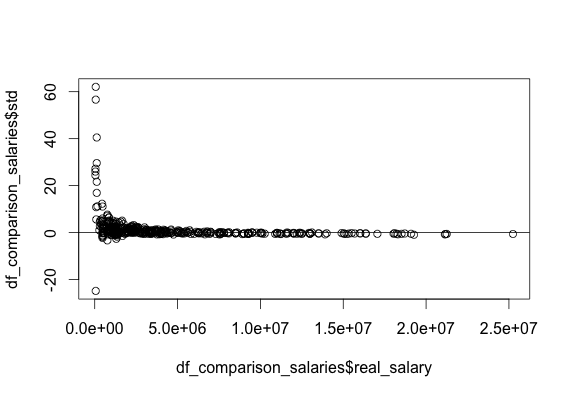
\includegraphics[width=0.75\textwidth]{images/Std_error}
\end{figure}
\\
We then plot the estimate salaries with the real salaries on the x axis. We can see that the coefficients we predicted are upper-bound for low salaries and lower-bound for high salaries.
\begin{figure}[h!]
\centering
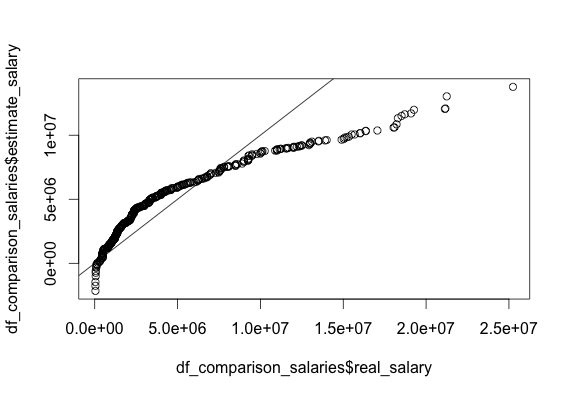
\includegraphics[width=0.75\textwidth]{images/Estimate_salaries}
\end{figure}

\paragraph{Salary causal analysis}Suppose we are interested in the effect of number of games played in a season have on salary. We can use differences-in-differences analysis. In a season, an increase in the number of games played would result in an increase in salary. We can investigate this by setting up a control group by creating a subset of data from 2004-2009. In the control group, we will have track variables such as Age, X3P, AST, TopPerformerWinShares. In the treatment group, we will create a subset of data from 2010-2014. The variables tracked will be the same as the control group, but we will include a new variable for the treatment group. We can then compare the average change of salary over time in the treatment group against average change of salary over time in the control group.

We assume the average change over the variables in the control group and treatment group cancels out each other. This removes the biases in comparison between the control and treatment groups.

\paragraph{Including corporation amongst members}We have collected player statistics that includes data that could give us an indication of how well a player does in a team setting or how much he contributes to the team’s success. In predicting player’s salaries, we can include variables that gives us an indication of teamwork and collaboration. Stats like points scored, minutes played usually indicate performance on an individual level.  Stats like number of assists (AST), field goal attempts (FGA), number of field goals/number of assists (FG/AST) usually indicate whether a player tends to shoot more or passes to a teammate in a better scoring position and bag the assist instead of points. If a player is not in the cluster of top players, his salary can be affected by his stats mentioned earlier. The higher those stats, he could be paid higher, compared to similar players but with lower stats in those areas.

\paragraph{Draft system: offer and supply}

\subparagraph{Which player a team chooses such that the player will accept?}Teams have to realize their reputation, or standings with other teams in the league. If a team is not popular, or always playing badly, they cannot expect to bid for a new athlete with the best stats and get their man. The new athlete usually have an idea of their abilities and the exceptional ones will be expecting big teams to come in with a hefty salary to get him on their team. Usually, smaller teams do not have the ability to pay that kind of money. Smaller teams should aim to entice players who are better than average and collaborate well with others in a team setting and develop them over the duration of their contracts. the probability for such players to accept an offer from a smaller team is also much higher.

\subparagraph{How much to initially offer a player?}We have to understand that overpaying for players will have repercussions in future. Not only will the salary become a drain for the team’s resources, the team is bound by contract to pay the salaries. Statistics can be collected on new athletes from their previous seasons before NBA, like NCAA, or previous leagues they come from. These data can be merged into the team’s own database so that comparisons between potential new recruits and current players playing in a similar position can be made. If the new athlete has similar stats than current players, the initial salary to offer to the new recruit will be 10-15\% lower than the average of the players he is compared to. This difference is because of the lack of experience of the potential new athlete. If the new athlete has better stats than current players playing in a similar position, the team can offer an initial salary to the new athlete that is comparable to the average salary of the players. This is to avoid the scenario where there is a big pay disparity between new players and current players of similar stats. The new athlete will have to understand that the team cannot overpay for players due to the wage structures in place. But if the athlete is of comparable ability than the rest of the team, he will be appropriately compensated for his services.

\subparagraph{Besides overpaying or underpaying a player, why else would a team reject a player?}A team can reject a player of he is not a fit to the team’s requirements (attempts many fields goals in a team with a lot of shooters, collect many rebounds in a team where it is already the case, etc). Also, a team may already have a lot of players in a particular position and the pool of new athletes have an excess of that position. For example, a team can have 4 power forwards, and the norm is that a team has 4 players in that position. So a team will not want add another power forward to its team roster and reject the player.
